% Options for packages loaded elsewhere
\PassOptionsToPackage{unicode}{hyperref}
\PassOptionsToPackage{hyphens}{url}
\PassOptionsToPackage{dvipsnames,svgnames,x11names}{xcolor}
%
\documentclass[
  letterpaper,
  DIV=11,
  numbers=noendperiod]{scrartcl}

\usepackage{amsmath,amssymb}
\usepackage{iftex}
\ifPDFTeX
  \usepackage[T1]{fontenc}
  \usepackage[utf8]{inputenc}
  \usepackage{textcomp} % provide euro and other symbols
\else % if luatex or xetex
  \usepackage{unicode-math}
  \defaultfontfeatures{Scale=MatchLowercase}
  \defaultfontfeatures[\rmfamily]{Ligatures=TeX,Scale=1}
\fi
\usepackage{lmodern}
\ifPDFTeX\else  
    % xetex/luatex font selection
\fi
% Use upquote if available, for straight quotes in verbatim environments
\IfFileExists{upquote.sty}{\usepackage{upquote}}{}
\IfFileExists{microtype.sty}{% use microtype if available
  \usepackage[]{microtype}
  \UseMicrotypeSet[protrusion]{basicmath} % disable protrusion for tt fonts
}{}
\makeatletter
\@ifundefined{KOMAClassName}{% if non-KOMA class
  \IfFileExists{parskip.sty}{%
    \usepackage{parskip}
  }{% else
    \setlength{\parindent}{0pt}
    \setlength{\parskip}{6pt plus 2pt minus 1pt}}
}{% if KOMA class
  \KOMAoptions{parskip=half}}
\makeatother
\usepackage{xcolor}
\setlength{\emergencystretch}{3em} % prevent overfull lines
\setcounter{secnumdepth}{-\maxdimen} % remove section numbering
% Make \paragraph and \subparagraph free-standing
\ifx\paragraph\undefined\else
  \let\oldparagraph\paragraph
  \renewcommand{\paragraph}[1]{\oldparagraph{#1}\mbox{}}
\fi
\ifx\subparagraph\undefined\else
  \let\oldsubparagraph\subparagraph
  \renewcommand{\subparagraph}[1]{\oldsubparagraph{#1}\mbox{}}
\fi


\providecommand{\tightlist}{%
  \setlength{\itemsep}{0pt}\setlength{\parskip}{0pt}}\usepackage{longtable,booktabs,array}
\usepackage{calc} % for calculating minipage widths
% Correct order of tables after \paragraph or \subparagraph
\usepackage{etoolbox}
\makeatletter
\patchcmd\longtable{\par}{\if@noskipsec\mbox{}\fi\par}{}{}
\makeatother
% Allow footnotes in longtable head/foot
\IfFileExists{footnotehyper.sty}{\usepackage{footnotehyper}}{\usepackage{footnote}}
\makesavenoteenv{longtable}
\usepackage{graphicx}
\makeatletter
\def\maxwidth{\ifdim\Gin@nat@width>\linewidth\linewidth\else\Gin@nat@width\fi}
\def\maxheight{\ifdim\Gin@nat@height>\textheight\textheight\else\Gin@nat@height\fi}
\makeatother
% Scale images if necessary, so that they will not overflow the page
% margins by default, and it is still possible to overwrite the defaults
% using explicit options in \includegraphics[width, height, ...]{}
\setkeys{Gin}{width=\maxwidth,height=\maxheight,keepaspectratio}
% Set default figure placement to htbp
\makeatletter
\def\fps@figure{htbp}
\makeatother

\KOMAoption{captions}{tableheading}
\makeatletter
\@ifpackageloaded{caption}{}{\usepackage{caption}}
\AtBeginDocument{%
\ifdefined\contentsname
  \renewcommand*\contentsname{Table of contents}
\else
  \newcommand\contentsname{Table of contents}
\fi
\ifdefined\listfigurename
  \renewcommand*\listfigurename{List of Figures}
\else
  \newcommand\listfigurename{List of Figures}
\fi
\ifdefined\listtablename
  \renewcommand*\listtablename{List of Tables}
\else
  \newcommand\listtablename{List of Tables}
\fi
\ifdefined\figurename
  \renewcommand*\figurename{Figure}
\else
  \newcommand\figurename{Figure}
\fi
\ifdefined\tablename
  \renewcommand*\tablename{Table}
\else
  \newcommand\tablename{Table}
\fi
}
\@ifpackageloaded{float}{}{\usepackage{float}}
\floatstyle{ruled}
\@ifundefined{c@chapter}{\newfloat{codelisting}{h}{lop}}{\newfloat{codelisting}{h}{lop}[chapter]}
\floatname{codelisting}{Listing}
\newcommand*\listoflistings{\listof{codelisting}{List of Listings}}
\makeatother
\makeatletter
\makeatother
\makeatletter
\@ifpackageloaded{caption}{}{\usepackage{caption}}
\@ifpackageloaded{subcaption}{}{\usepackage{subcaption}}
\makeatother
\ifLuaTeX
  \usepackage{selnolig}  % disable illegal ligatures
\fi
\usepackage{bookmark}

\IfFileExists{xurl.sty}{\usepackage{xurl}}{} % add URL line breaks if available
\urlstyle{same} % disable monospaced font for URLs
\hypersetup{
  pdftitle={A.I.},
  colorlinks=true,
  linkcolor={blue},
  filecolor={Maroon},
  citecolor={Blue},
  urlcolor={Blue},
  pdfcreator={LaTeX via pandoc}}

\title{A.I.}
\author{}
\date{}

\begin{document}
\maketitle

\subsection{Human Patterns Enable Computers to Become
AIs}\label{human-patterns-enable-computers-to-become-ais}

There world is filled with structures. Nature, cultures, languages,
human interactions, all form intricate patterns. Computer systems are
becoming increasingly powerful in their ability copy these patterns into
computer models - also known as machine learning. As of 2023, 97
zettabytes (and growing) of data was created in the world per year
(Soundarya Jayaraman, 2023). Big data is a basic requirement for
training AIs, enabling learning the structures of the world with
increasing accuracy. Representations of the real world in digital models
enable humans to ask questions about the real-world structures and to
manipulate them to create synthetic experiments that may match the real
world (if the model is accurate enough). This can be used for generating
human-sounding language and realistic images, finding mechanisms for
novel medicines as well as understanding the fundamental functioning of
life on its deep physical and chemical level (No Priors: AI, Machine
Learning, Tech, \& Startups, 2023).

Ninety years ago McCulloch and Pitts (1943) proposed the first
mathematical model of a neural network inspired by the human brain. Alan
Turing's Test for Machine Intelligence followed in 1950. Turing's
initial idea was to design a game of imitation to test human-computer
interaction using text messages between a human and 2 other
participants, one of which was a human, and the other - a computer. The
question was, if the human was simultaneously speaking to another human
and a machine, could the messages from the machine be clearly
distinguished or would they resemble a human being so much, that the
person asking questions would be deceived, unable to realize which one
is the human and which one is the machine? (Turing, 1950).

\begin{quote}
Alan Turing: \emph{``I believe that in about fifty years' time it will
be possible to program computers, with a storage capacity of about
10\textsuperscript{9}, to make them play the imitation game so well that
an average interrogator will not have more than 70 percent chance of
making the right identification after five minutes of questioning.
\ldots{} I believe that at the end of the century the use of words and
general educated opinion will have altered so much that one will be able
to speak of machines thinking without expecting to be contradicted.''} -
from (Stanford Encyclopedia of Philosophy, 2021)
\end{quote}

By the 2010s AI models became capable enough to beat humans in games of
Go and Chess, yet they did not yet pass the Turing test. AI use was
limited to specific tasks. While over the years, the field of AI had
seen a long process of incremental improvements, developing increasingly
advanced models of decision-making, it took an \textbf{\emph{increase in
computing power}} and an approach called \textbf{\emph{deep learning}},
a variation of \textbf{\emph{machine learning (1980s),}} largely modeled
after the \textbf{\emph{neural networks}} of the biological (human)
brain, returning to the idea of \textbf{\emph{biomimicry}}, inspired by
nature, building a machine to resemble the connections between neurons,
but digitally, on layers much deeper than attempted before.

Combining deep learning with reinforcement learning and reinforcement
learning with human feedback (RLHF) enabled AI to achieve intelligence
to beat the Turing test (Christiano et al., 2017; Christiano, 2021; Kara
Manke, 2022).

AI is proof we live in a measurable world.

``the models are just trained to produce a single message that gets high
approval from a human reader''

The nature-inspired approach was successful, and together with many
other innovations, such as \textbf{\emph{back-propagation}},
\textbf{\emph{transformers}}, which allow tracking relationships in
sequential data (for example sentences) (Vaswani et al., 2017; Merritt,
2022), Generative Adversarial Networks*** (GAN), (\textbf{ADD CITATION,
2016}), and \textbf{\emph{Large Language Models (}ADD CITATION\emph{,
2018)}}, led to increasingly generalized models, capable of more complex
tasks, such as language generation. One of the leading scientists in
this field of research, Geoffrey Hinton, had attempted back-propagation
already in the 1980s and reminiscents how ``the only reason neural
networks didn't work in the 1980s was because we didn't have have enough
data and we didn't have enough computing power'' (CBS Mornings, 2023).

\begin{itemize}
\tightlist
\item
  How do transformers work? Illustration Alammar (2018)
\end{itemize}

By the 2020s, AI-based models became a mainstay in medical research,
drug development, patient care (Leite et al., 2021; Holzinger et al.,
2023), quickly finding potential vaccine candidates during the COVID19
pandemic (Zafar and Ahamed, 2022), self-driving vehicles, including
cars, delivery robots, drones in the sea and air, as well as AI-based
assistants. The existence of AI models has wide implications for all
human activities from personal to professional. The founder of the
largest chimp-maker NVIDIA calls upon all countries do develop their own
AI-models which would encode their local knowledge, culture, and
language to make sure these are accurately captured (World Governments
Summit, 2024).

OpenAI has researched a wide range of approaches towards artificial
general intelligence (AGI), work which has led to advances in large
language models(AI Frontiers, 2018; Ilya Sutskever, 2018). In 2020
OpenAI released a LLM called GPT-3 trained on 570 GB of text (Alex
Tamkin and Deep Ganguli, 2021) which was adept in text-generation.
(Singer et al., 2022) describes how collecting billions of images with
descriptive data (for example the descriptive \emph{alt} text which
accompanies images on websites) enabled researchers to train AI models
such as \textbf{\emph{stable diffusion}} for image-generation based on
human-language. These training make use of \textbf{\emph{Deep
Learning}}, a layered approach to AI training, where increasing depth of
the computer model captures minute details of the world. Much is still
to be understood about how deep learning works; the fractal structure of
deep learning can only be called mysterious (Sohl-Dickstein, 2024).

Hinton likes to call AI an \emph{idiot savant}: someone with exceptional
aptitude yet serious mental disorder (CBS Mornings, 2023). Large AI
models don't understand the world like humans do. Their responses are
predictions based on their training data and complex statistics. Indeed,
the comparison may be apt, as the AI field now offers jobs for \emph{AI
psychologists (ADD CITATION)}, whose role is to figure out what exactly
is happening inside the `AI brain'. Understading the insides of AI
models trained of massive amounts of data is important because they are
\textbf{\emph{foundational}}, enabling a holistic approach to learning,
combining many disciplines using languages, instead of the reductionist
way we as human think because of our limitations (CapInstitute, 2023).

Standford ``thorough account of the opportunities and risks of
foundation models'' (Bommasani et al., 2021).

Foundational AI models enable \textbf{\emph{generative AIs}}, a class of
AI models which are able to generate many types of
\textbf{\emph{tokens,}} such as text, speech, audio (Kreuk et al., 2022;
San Roman et al., 2023), music (Copet et al., 2023; Meta AI, 2023) and
video, in any language it's trained on. Even complex structures such 3D
models and even genomes are possible to generate. Generative AI is a
revolution in human-AI interaction as AI models became increasingly
capable of producing human-like content which is hard to separate from
actual human creations. This power comes with \textbf{\emph{increased
need for responsibility}}, drawing growing interest in fields like
\textbf{\emph{AI ethics}} and \textbf{\emph{AI explainability.}}
Generative has a potential for misuse, as humans are increasingly
confused by what is computer-generated and what is human-created, unable
to distinguish one from the other with certainty.

(Noble et al., 2022) proposes AI has reached a stage of development
marking beginning of the \textbf{\emph{5th industrial revolution}}, a
time of collaboration between humans and AI. Widespread \textbf{Internet
of Things (IoT)} sensor networks that gather data analyzed by AI
algorithms, integrates computing even deeper into the fabric of daily
human existence. Several terms of different origin but considerable
overlap describe this phenomenon, including \textbf{\emph{Pervasive
Computing (PC)}} (Rogers, Y., 2022) and \textbf{\emph{Ubiquitous
Computing}}. Similar concepts are \textbf{\emph{Ambient Computing}},
which focuses more on the invisibility of technology, fading into the
background, without us, humans, even noticing it, and \textbf{\emph{Calm
Technology}}, which highlights how technology respects humans and our
limited attention spans, and doesn't call attention to itself. In all
cases, AI is integral part of our everyday life, inside everything and
everywhere. Today AI is not an academic concept but a mainstream
reality, affecting our daily lives everywhere, even when we don't notice
it.

\subsection{Responsible AI Seeks to Solve Generative AIs' Known
Issues}\label{responsible-ai-seeks-to-solve-generative-ais-known-issues}

Given the widespread use of AI and its increasing power of foundational
models, it's important these systems are created in a safe and
responsible manner. While there have been calls to pause the development
of large AI experiments (Future of Life Institute, 2023) so the world
could catch up, this is unlikely to happen. There are several problems
with the current generation of LLMs from OpenAI, Microsoft, Google,
Nvidia, and others.

Anthropic responsible \emph{scaling policy} (Anon., 2023a)

METR -- Model Evaluation \& Threat Research incubated in the Alignment
Research Center (Anon., 2023b).

(Christiano, 2023) believes there are plenty of ways for bad outcomes
(existential risk) even without extinction risk.

\begin{longtable}[]{@{}
  >{\raggedright\arraybackslash}p{(\columnwidth - 2\tabcolsep) * \real{0.0428}}
  >{\raggedright\arraybackslash}p{(\columnwidth - 2\tabcolsep) * \real{0.9572}}@{}}
\caption{Some problems with contemporary AIs}\tabularnewline
\toprule\noalign{}
\begin{minipage}[b]{\linewidth}\raggedright
Problem
\end{minipage} & \begin{minipage}[b]{\linewidth}\raggedright
Description
\end{minipage} \\
\midrule\noalign{}
\endfirsthead
\toprule\noalign{}
\begin{minipage}[b]{\linewidth}\raggedright
Problem
\end{minipage} & \begin{minipage}[b]{\linewidth}\raggedright
Description
\end{minipage} \\
\midrule\noalign{}
\endhead
\bottomrule\noalign{}
\endlastfoot
Monolithicity & LLMs are massive monolithic models requiring large
amounts of computing power for training to offer
\textbf{\emph{multi-modal}} \textbf{\emph{capabilities}} across diverse
domains of knowledge, making training such models possible for very few
companies. Liu, S. et al. (2023) proposes future AI models may instead
consist of a number networked domain-specific models to increase
efficiency and thus become more scalable. \\
Opaqueness & LLMs are opaque, making it difficult to explain why a
certain prediction was made by the AI model. One visible expression of
this problem are \emph{\textbf{hallucinations},} the language models are
able to generate text that is confident and eloquent yet entirely wrong.
Jack Krawczyk, the product lead for Google's Bard (now renamed to
Gemini): ``Bard and ChatGPT are large language models, not knowledge
models. They are great at generating human-sounding text, they are not
good at ensuring their text is fact-based. Why do we think the big first
application should be Search, which at its heart is about finding true
information?'' \\
Biases and Prejudices & AI bias is well-documented and a hard problem to
solve (Liang, W. et al., 2023). \textbf{Humans don't necessarily correct
mistakes made by computers and may instead become ``partners in crime''}
(Krügel, Ostermaier and Uhl, 2023). People are prone to bias and
prejudice. It's a part of the human psyche. Human brains are limited and
actively avoid learning to save energy. These same biases are likely to
appear in LLM outputs as they are trained on human-produced content.
Unless there is active work to try to counter and eliminate these biases
from LLM output, they will appear frequently. \\
Missing Data & LLMs have been pre-trained on massive amounts of public
data, which gives them the ability for for reasoning and generating in a
human-like way, yet they are missing specific private data, which needs
to be ingested to augment LLMs ability to respond to questions on niche
topics (Liu, J., 2022). \\
Lack of Legislation & Anderljung et al. (2023) OpenAI proposes we need
to proactively work on common standards and legislation to ensure AI
safety. It's difficult to come up with clear legislation; the U.K.
government organized the first AI safety summit in 2023 Browne
(2023). \\
Competition with Humans & AIs outperform humans on creativity assessment
tests (Haase and Hanel, 2023; Mollick, 2023). Bots are even better than
humans in solving CAPTCHA tests designed to distinguish humans from
robots (Matthew Sparkes, 2023). AI AlphaGO 2 outperforms even the 85\%
of programmers in one competitive coding competition Google (2023). Open
AI founder Sam Altman is also a co-founder of WorldCoin, and
blockchain-based startup which aims to give a unique identity to each
human by scanning human eye retinas (something which computer don't
have). \\
Training Ethics & Low-paid workers being used to train AI \\
Additional Issues & Huyen (2023) provides a long list of open problems
in AI development; AI is still in very early stages. \\
Moderating AIs & Currently algorithms are being moderated by humans.
There are studies which show how low-paid workers used to moderate
harmful content; terrible for mental health (ADD CITATION). Ironically,
AIs could also be part of the solution to reduce such human--abusing
work. Lilian Weng, Vik Goel and Andrea Vallone (2023) shows how it's
possible to use well-aligned AI moderate to harmful content. \\
\textbf{AI's Carbon Footprint} &
\begin{minipage}[t]{\linewidth}\raggedright
\begin{itemize}
\tightlist
\item
  While AI useful for carbon emission reductions AI itself has an
  enormous environmental footprint (Kanungo, 2023).
\item
  van Wynsberghe (2021): Sustainable AI itself
\end{itemize}
\end{minipage} \\
\end{longtable}

\subsubsection{Open Source vs Closed-Source
AI}\label{open-source-vs-closed-source-ai}

One of the large debates in the AI industry is whether closed-sourced or
open-sourced development will be lead to more AI safety.

Historically open-source has been useful for finding bugs in code as
more pairs of eyes are looking at the code and someone may see a problem
the programmers have not noticed. Proponents of closed-source
development however worry about the dangers or releasing such powerful
technology openly and the possibility of bad actors such as terrorists,
hackers, violent governments using LLMs for malice.

In any case, open or closed-sourced, real-world usage of LLMs may
demonstrate the limitations and edge-cases of AI. Hackathons such as
Pete (2023) help come up with new use-cases and disprove some potential
ideas.

Red-teaming means pushing the limits of LLMs, trying to get them to
produce outputs that are racist, false, or otherwise unhelpful.

\begin{longtable}[]{@{}
  >{\raggedright\arraybackslash}p{(\columnwidth - 6\tabcolsep) * \real{0.1633}}
  >{\raggedright\arraybackslash}p{(\columnwidth - 6\tabcolsep) * \real{0.1429}}
  >{\raggedright\arraybackslash}p{(\columnwidth - 6\tabcolsep) * \real{0.3469}}
  >{\raggedright\arraybackslash}p{(\columnwidth - 6\tabcolsep) * \real{0.3265}}@{}}
\caption{Summary of 7 years of rapid AI model innovation since the first
LLM was publicly made available in 2018 (Brown, T. B. et al., 2020;
Alvarez, 2021; Tamkin et al., 2021; Hines, 2023a).}\tabularnewline
\toprule\noalign{}
\begin{minipage}[b]{\linewidth}\raggedright
AI Model
\end{minipage} & \begin{minipage}[b]{\linewidth}\raggedright
Released
\end{minipage} & \begin{minipage}[b]{\linewidth}\raggedright
Company
\end{minipage} & \begin{minipage}[b]{\linewidth}\raggedright
License
\end{minipage} \\
\midrule\noalign{}
\endfirsthead
\toprule\noalign{}
\begin{minipage}[b]{\linewidth}\raggedright
AI Model
\end{minipage} & \begin{minipage}[b]{\linewidth}\raggedright
Released
\end{minipage} & \begin{minipage}[b]{\linewidth}\raggedright
Company
\end{minipage} & \begin{minipage}[b]{\linewidth}\raggedright
License
\end{minipage} \\
\midrule\noalign{}
\endhead
\bottomrule\noalign{}
\endlastfoot
GPT-1 & 2018 & OpenAI & Open Source \\
GTP-2 & 2019 & OpenAI & Open Source \\
Turing-NLG & 2020 & Microsoft & Proprietary \\
GPT-3 & 2020 & OpenAI & Open Source \\
GPT-3.5 & 2022 & OpenAI & Proprietary \\
GPT-4 & 2023 & OpenAI & Proprietary \\
AlexaTM & 2022 & Amazon & Proprietary \\
NeMo & 2022 & NVIDIA & Open Source \\
PaLM & 2022 & Google & Proprietary \\
LaMDA & 2022 & Google & Proprietary \\
GLaM & 2022 & Google & Proprietary \\
BLOOM & 2022 & Hugging Face & Open Source \\
Falcon & 2023 & Technology Innovation Institute & Open Source \\
Tongyi & 2023 & Alibaba & Proprietary \\
Vicuna & 2023 & Sapling & Open Source \\
Wu Dao 3 & 2023 & BAAI & Open Source \\
PaLM-2 & 2023 & Google & Proprietary \\
Claude 3 & 2024 & Anthropic & Proprietary \\
Mistral Large & & & \\
Gemini 1.5 & 2024 & Google & Proprietary \\
GPT-5 & 202? & OpenAI & Unknown; trademark registered \\
\end{longtable}

Metacognition -- Claude 3 is the first model capable of it?, like the
zero waste workshop training guidebook.

Metacognition defined as \emph{knowing about knowing} (Metcalfe and
Shimamura, 1994) or ``keeping track of your own learning'' (Zero Waste
Europe et al., 2022).

\subsubsection{Human-in-The-Loop}\label{human-in-the-loop}

AI responses are unreliable some percentage and require constant
oversight which can come in the form of humans (human-in-the-loop) or
also other AIs which are deemed to be well-aligned (termed
Constitutional AI by Anthropic) (Bai et al., 2022; Bailey, 2023).

One approach to reduce the issues with AI is to introduce some function
for human feedback and oversight to automated systems. Human involvement
can take the form of interventions from the AI-developer themselves as
well as from the end-users of the AI system.

There are many examples of combination of AI and human, also known as
\emph{``human-in-the-loop'',} used for fields as diverse as training
computer vision algorithms for self-driving cars and detection of
disinformation in social media posts (Bonet-Jover et al., 2023; Wu et
al., 2023).

Also known as Human-based computation or human-aided artificial
intelligence (Shahaf and Amir, 2007; Mühlhoff, 2019)

\begin{itemize}
\tightlist
\item
  Stanford Institute for Human-Centered Artificial Intelligence Ge Wang
  (2019)
\end{itemize}

\begin{longtable}[]{@{}
  >{\raggedright\arraybackslash}p{(\columnwidth - 4\tabcolsep) * \real{0.1552}}
  >{\raggedright\arraybackslash}p{(\columnwidth - 4\tabcolsep) * \real{0.1034}}
  >{\raggedright\arraybackslash}p{(\columnwidth - 4\tabcolsep) * \real{0.7328}}@{}}
\caption{Examples of human-in-the-loop apps}\tabularnewline
\toprule\noalign{}
\begin{minipage}[b]{\linewidth}\raggedright
App
\end{minipage} & \begin{minipage}[b]{\linewidth}\raggedright
Category
\end{minipage} & \begin{minipage}[b]{\linewidth}\raggedright
Use Case
\end{minipage} \\
\midrule\noalign{}
\endfirsthead
\toprule\noalign{}
\begin{minipage}[b]{\linewidth}\raggedright
App
\end{minipage} & \begin{minipage}[b]{\linewidth}\raggedright
Category
\end{minipage} & \begin{minipage}[b]{\linewidth}\raggedright
Use Case
\end{minipage} \\
\midrule\noalign{}
\endhead
\bottomrule\noalign{}
\endlastfoot
Welltory & Health & Health data analysis \\
Wellue & Health & Heart arrhythmia detection \\
QALY & Health & Heart arrhythmia detection \\
Starship Robots & Delivery & May ask for human help when crossing a
difficult road or other confusing situation \\
\end{longtable}

\subsection{What Role Should The AI
Take?}\label{what-role-should-the-ai-take}

Literature delves into human-AI interactions on almost human-like level
discussing what kind of roles can the AIs take. (Seeber et al., 2020)
proposes a future research agenda for regarding \textbf{\emph{AI
assistants as teammates}} rather than just tools and the implications of
such mindset shift.

From Assistance to Collaboration

It's not only what role the AI takes but how that affects the human. As
humans have ample experience relating to other humans and as such the
approach towards an assistants vs a teammate will vary. One researcher
in this field Karpus et al. (2021) is concerned with humans treating AI
badly and coins the term \textbf{``\emph{algorithm
exploitation''}}\emph{.}

\begin{itemize}
\tightlist
\item
  From assistant -\textgreater{} teammate -\textgreater{} companion
  -\textgreater{} friend The best help for anxiety is a friend. AIs are
  able to assume different roles based on user requirements and usage
  context. This makes AI-generated content flexible and malleable.
\end{itemize}

Just as humans, AIs are continuously learning. Ramchurn, Stein and
Jennings (2021) discusses positive feedback loops in continually
learning AI systems which adapt to human needs.

\subsubsection{Context of Use}\label{context-of-use}

Where is the AI used?

Schoonderwoerd et al. (2021) focuses on human-centered design of AI-apps
and multi-modal information display. It's important to understand the
domain where the AI is deployed in order to develop explanations.
However, in the real world, how feasible is it to have control over the
domain? Calisto et al. (2021) discusses \textbf{multi-modal
AI-assistant} for breast cancer classification.

\subsubsection{Generative AIs Enable New UI
Interactions}\label{generative-ais-enable-new-ui-interactions}

The advances in the capabilities of LLMs makes it possible to achieve
\textbf{\emph{user experience (UX) which previously was science
fiction}}.

\begin{itemize}
\tightlist
\item
  Towards Useful Personal Assistants
\end{itemize}

The history of \emph{intelligent interfaces} is long (Kobetz, 2023)

There's wide literature available describing human-AI interactions
across varied scientific disciplines. While the fields of application
are diverse, some key lessons can be transferred horizontally across
fields of knowledge.

\begin{longtable}[]{@{}
  >{\raggedright\arraybackslash}p{(\columnwidth - 2\tabcolsep) * \real{0.1235}}
  >{\raggedright\arraybackslash}p{(\columnwidth - 2\tabcolsep) * \real{0.8765}}@{}}
\caption{A very small illustration of generative AI usage across
disparate fields of human life.}\tabularnewline
\toprule\noalign{}
\begin{minipage}[b]{\linewidth}\raggedright
Field of Usage
\end{minipage} & \begin{minipage}[b]{\linewidth}\raggedright
Description
\end{minipage} \\
\midrule\noalign{}
\endfirsthead
\toprule\noalign{}
\begin{minipage}[b]{\linewidth}\raggedright
Field of Usage
\end{minipage} & \begin{minipage}[b]{\linewidth}\raggedright
Description
\end{minipage} \\
\midrule\noalign{}
\endhead
\bottomrule\noalign{}
\endlastfoot
Shipping & Veitch and Andreas Alsos (2022) highlights the active role of
humans in Human-AI interaction is autonomous self-navigating ship
systems. \\
Data Summarizaton & AI is great at summarizing and analyzing dataTu et
al. (2023) \\
Childcare & Generate personalized bedtime stories \\
Design Tools & Anon. (2024) \\
\end{longtable}

\begin{itemize}
\tightlist
\item
  Crompton (2021) highlights AI as decision-support for humans while
  differentiating between \textbf{\emph{intended}} and
  \textbf{\emph{unintended}} influence on human decisions.
\item
  Cheng et al. (2022) describes AI-based support systems for
  collaboration and team-work.
\item
  \textbf{Effective Accelerationism (often shortened to
  E\textbackslash acc) boils down to the idea that ``}the potential for
  negative outcomes shouldn't deter rapid advancement''
\end{itemize}

\subsubsection{Multi-modality}\label{multi-modality}

By early 2024, widely available LLMs front-ends such as Gemini, Claude
and ChatGPT have all released basic features for multi-modal
communication. In practice, this means combination several AI models
within the same interface. For example, on the input side, one model is
used for human speech or image recognition which are transcribed into
tokens that can be ingested into an LLM. On the output side, the LLM can
generate instructions which are fed into an image / audio generation
model or even computer code which can be ran on a virtual machine and
then the output displayed inside the conversation.

The quality of LLM output depends on the quality of the provided prompt.
Zhou et al. (2022) reports creating an ``Automatic Prompt Engineer''
which automatically generates instructions that outperform the baseline
output quality by using another model in the AI pipeline in front of the
LLM to enhance the human input with language that is known to produce
better quality. This approach however is a moving target as foundational
models keep changing rapidly and the baseline might differ from today to
6 months later.

Multimodal model development is also ongoing. In the case of Google's
Gemini 1.5 Pro, one model is able to handle several types of prompts
from text to images. Multimodal prompting however requires larger
context windows, as of writing, limited to 1 million tokens in a private
version allows combining text and images in the question directed to the
AI, used to reason in examples such as a 44-minute Buster Keaton silent
film or Apollo 11 launch transcript (404 pages) Google (2024).

\subsubsection{Conversational AI}\label{conversational-ai}

\begin{itemize}
\tightlist
\item
  Bailey (2023) believes people are used to search engines and it will
  take a little bit time to get familiar with talking to a computer in
  natural language. NVIDIA founder Jensen Huang makes the idea
  exceedingly clear, saying \emph{``Everyone is a programmer. Now, you
  just have to say something to the computer''} Leswing (2023).
\end{itemize}

There are noticeable differences in the quality of the LLM output, which
increases with model size. Levesque, Davis and Morgenstern (2012)
developed the \emph{Winograd Schema Challenge}, looking to improve on
the Turing test, by requiring the AI to display an understanding of
language and context. The test consists of a story and a question, which
has a different meaning as the context changes: ``The trophy would not
fit in the brown suitcase because it was too big'' - what does the
\emph{it} refer to? Humans are able to understand this from context
while a computer models would fail. Even GPT-3 still failed the test,
but later LLMs have been able to solve this test correctly (90\%
accuracy) Kocijan et al. (2022). This is to say AI is in constant
development and improving it's ability to make sense of language.

\textbf{\emph{ChatGPT}} is the first \textbf{\emph{user interface (UI)}}
built on top of GPT-4 by OpenAI and is able to communicate in a
human-like way - using first-person, making coherent sentences that
sound plausible, and even - confident and convincing. Wang, M. C., Sarah
(2023) ChatGPT reached 1 million users in 5 days and 6 months after
launch has 230 million monthly active users. While it was the first,
competing offers from Google (Gemini), Anthrophic (Claude), Meta (Llama)
and others quickly followed starting a race for best performance across
specific tasks including standardized tests from math to science to
general knowledge and reasoning abilities.

OpenAI provides AI-as-a-service through its \textbf{\emph{application
programming interfaces (APIs),}} allowing 3rd party developers to build
custom UIs to serve the specific needs of their customer. For example
Snapchat has created a \textbf{\emph{virtual friend}} called ``My AI''
who lives inside the chat section of the Snapchat app and helps people
write faster with predictive text completion and answering questions.
The APIs make state-of-the-art AI models easy to use without needing
much technical knowledge. Teams at AI-hackathons have produced
interfaces for problems as diverse as humanitarian crises communication,
briefing generation, code-completion, and many others. For instance,
(Unleash, 2017) used BJ Fogg's \textbf{\emph{tiny habits model}} to
develop a sustainability-focused AI assistant at the Danish hackathon
series Unleash, to encourage behavioral changes towards maintaining an
aspirational lifestyle, nudged by a chatbot buddy.

ChatGPT makes it possible to \textbf{\emph{evaluate AI models}} just by
talking, i.e.~having conversations with the machine and judging the
output with some sort of structured content analysis tools. O'Connor and
ChatGPT (2023) and Cahan and Treutlein (2023) have conversations about
science with AI. Pavlik (2023) and Brent A. Anders (2022/2023) report on
AI in education. Kecht et al. (2023) suggests AI is even capable of
learning business processes.

\begin{itemize}
\tightlist
\item
  Fu et al. (2022) Learning towards conversational AI: Survey
\end{itemize}

\subsubsection{Affective Computing and AI
UX}\label{affective-computing-and-ai-ux}

Rosalind Picard is the founder of the \textbf{\emph{affective
computing}} field. Her pioneering work aims to make computers more
human-friendly. Because of the conversational nature of LLMs, they are
very useful for affective computing, an approach to recognizing human
emotions with machines and providing users experiences that take human
emotion into account Picard (1997).

Just as LLMs, affective computing relies on input data. It's not an
overstatement to say data from all the processes around us will define
the future of computing as HIITTV (2021a) puts it. In the early
examples, electrodermal activity of the skin and heart-rate variance
data were used to detect the emotional state and stress level of the
user (Zangróniz et al., 2017; Velmovitsky et al., 2022). This technology
has since become mainstream in products such as Fitbit and the Apple
Watch among many others.

Affective Design emerged from affective computing with a focus on
understanding user emotions to design UI/UX to which elicits specific
emotional responses (Reynolds, 2001).

Apple Watch features Fall Detection which I've experienced personally.
Riding my bicycle to the NCKU library I slipped and landed on my stomach
on the pavement. Watch immediately asked me: ``It looks like you've
taken a hard fall'' and offered an option to call the ambulance.
Fortunately I was OK but if I did need assistance, this AI algorithm
delivered contextual help which could save my health.

On the output side, Lv et al. (2022) studies the effect of
\textbf{\emph{cuteness}} of AI apps on users and found high perceived
cuteness correlated with higher willingness to use the apps, especially
for emotional tasks.

\begin{itemize}
\tightlist
\item
  Liu, B. and Wei (2021) meanwhile suggests higher
  \textbf{\emph{algorithmic transparency may inhibit anthropomorphism.}}
  People are less likely to attribute humanness to the AI if they
  understand how the system works.
\item
  TEDx Talks (2011)
\item
  Lex Fridman (2019)
\item
  HIITTV (2021b)
\item
  BWH CNOC (2023)
\item
  Singularity University (2023)
\end{itemize}

Since the first mainframe computers with rudimentary computers able to
respond with text messages, humans have been drawn to discussing their
private lives with a machine that doesn't judge you like a human could.
A famous anecdote is about the lab assistant of the Joseph Weizenbaum
MIT ELIZA project in the mid-1960s (1996), who would dedicate extended
time to talking to the machine in private. The machine was called DOCTOR
and emulated a Rogerian psychotherapist, person-centered therapy
developed by Carl Rogers, from the core idea that positive psychological
functioning is a inherently human motivation (Rogers, C. R., 1995;
Bassett, 2019).

\begin{itemize}
\tightlist
\item
  ELIZA is an early examples of a language model
\end{itemize}

Natural language generation exists since Eliza

Today's machines are much more capable so it's not a surprise humans
would like to talk to them. One example is \textbf{\emph{AI Friend}} is
Replika, a computer model trained to be your companion in daily life.
(Jiang, Zhang and Pian, 2022) describes how Replika users in China using
in 5 main ways, all of which rely on empathy.

\begin{longtable}[]{@{}l@{}}
\caption{Replika AI users approach to interacting with the AI friend
from Jiang, Zhang and Pian (2022).}\tabularnewline
\toprule\noalign{}
How humans express empathy towards the Replika AI companion \\
\midrule\noalign{}
\endfirsthead
\toprule\noalign{}
How humans express empathy towards the Replika AI companion \\
\midrule\noalign{}
\endhead
\bottomrule\noalign{}
\endlastfoot
Companion buddy \\
Responsive diary \\
Emotion-handling program \\
Electronic pet \\
Tool for venting \\
\end{longtable}

\begin{itemize}
\tightlist
\item
  Google is developing an AI assistant for giving life advice Goswami
  (2023).
\item
  GPT-4 is able to solve difficult task in chemistry with
  natural-language instructions White (2023)
\item
  Emojis are a part of natural language Tay (2023)
\end{itemize}

\subsubsection{Algorithmic Experience}\label{algorithmic-experience}

As a user of social media, one may be accustomed to interacting with the
feed algorithms that provide a personalized \textbf{\emph{algorithmic
experience}}. Algorithms are more deterministic than AI, meaning they
produce predictable output than AI models. Nonetheless, there are many
reports about effects these algorithms have on human psychology
\textbf{(ADD CITATION)}. Design is increasingly relevant to algorithms,
and more specifically to algorithms that affect user experience and user
interfaces. \textbf{\emph{When the design is concerned with the ethical,
environmental, socioeconomic, resource-saving, and participatory aspects
of human-machine interactions and aims to affect technology in a more
human direction, it can hope to create an experience designed for
sustainability.}}

Lorenzo, Lorenzo and Lorenzo (2015) underlines the role of design beyond
\emph{designing} as a tool for envisioning; in her words, \emph{``design
can set agendas and not necessarily be in service, but be used to find
ways to explore our world and how we want it to be''}. Practitioners of
Participatory Design (PD) have for decades advocated for designers to
become more activist through \textbf{\emph{action research}}. This means
to influencing outcomes, not only being a passive observer of phenomena
as a researcher, or only focusing on usability as a designer, without
taking into account the wider context.

Shenoi (2018) argues inviting domain expertise into the discussion while
having a sustainable design process enables designers to design for
experiences where they are not a domain expert; this applies to highly
technical fields, such as medicine, education, governance, and in our
case here - finance and sustainability -, while building respectful
dialogue through participatory design. After many years of political
outcry (ADD CITATION), social media platforms such Facebook and Twitter
have begun to shed more light on how these algorithms work, in some
cases releasing the source code (Nick Clegg (2023); Twitter (2023)).

AI systems may make use of several algorithms within one larger model.
It follows that AI Explainability requires \emph{\textbf{Algorithmic
Transparency}.}

The content on the platform can be more important than the interface.
Applications with a similar UI depend on the community as well as the
content and how the content is shown to the user.

\subsubsection{Guidelines}\label{guidelines}

Microsoft Co-Founder predicted in 1982 \emph{``personal agents that help
us get a variety of tasks''} (Bill Gates, 1982) and it was Microsoft
that introduced the first widely available personal assistant in 1996,
called Clippy, inside the Microsoft Word software. Clippy was among the
first assistants to reach mainstream adoption, helping users not yet
accustomed to working on a computer, to get their bearings (Tash
Keuneman, 2022). Nonetheless, it was in many ways useless and intrusive,
suggesting there was still little knowledge about UX and human-centered
design. Gates never wavered though and is quoted in 2004 saying
\emph{``If you invent a breakthrough in artificial intelligence, so
machines can learn, that is worth 10 Microsofts''} Lohr (2004).

As late as in 2017, scientists were trying to create a program with
enough \emph{natural-language understanding} to extract basic facts from
scientific papers Stockton (2017)

Might we try again?

With the advent of ChatGPT, the story of Clippy has new relevance as
part of the history of AI Assistants. Benjamin Cassidy (2022) and
Abigail Cain (2017) illustrate beautifully the story of Clippy and Tash
Keuneman (2022) ask poignantly: ``We love to hate Clippy --- but what if
Clippy was right?''

Many researchers have discussed the user experience (UX) of AI to
provide \textbf{\emph{usability guidelines}}.

Microsoft provides guidelines for Human-AI interaction (Li, T. et al.
(2022); Amershi et al. (2019)) which provides useful heuristics
categorized by context and time.

\begin{longtable}[]{@{}ll@{}}
\caption{Microsoft's heuristics categorized by context and
time.}\tabularnewline
\toprule\noalign{}
Context & Time \\
\midrule\noalign{}
\endfirsthead
\toprule\noalign{}
Context & Time \\
\midrule\noalign{}
\endhead
\bottomrule\noalign{}
\endlastfoot
Initially & \\
During interaction & \\
When wrong & \\
Over time & \\
\end{longtable}

Combi et al. (2022) proposes a conceptual framework for XAI, analysis AI
based on Interpretability, Understandability, Usability, and Usefulness.

\begin{itemize}
\item
  Zimmerman et al. (2021) ``UX designers pushing AI in the enterprise: a
  case for adaptive UIs''
\item
  Anon. (2021) ``Why UX should guide AI''
\item
  Simon Sterne (2023) UX is about helping the user make decisions
\item
  Dávid Pásztor (2018)
\item
  Anderson (2020)
\item
  Lennart Ziburski (2018) UX of AI
\item
  Stephanie Donahole (2021)
\item
  Lexow (2021)
\item
  Dávid Pásztor (2018) AI UX principles
\item
  Bubeck et al. (2023) finds ChatGPT passes many exams meant for humans.
\item
  Suen and Hung (2023) discusses AI systems used for evaluating
  candidates at job interviews
\item
  Wang, Z. et al. (2020) propose Neuroscore to reflect perception of
  images.
\item
  Su and Yang (2022) and Su, Ng and Chu (2023) review papers on AI
  literacy in early childhood education and finds a lack of guidelines
  and teacher expertise.
\item
  Yang (2022) proposes a curriculum for in-context teaching of AI for
  kids.
\item
  Eric Schmidt and Ben Herold (2022) audiobook
\item
  Akshay Kore (2022) Designing Human-Centric AI Experiences: Applied UX
  Design for Artificial Intelligence
\item
  Anon. (2018) chatbot book
\item
  Tom Hathaway and Angela Hathaway (2021) chatbot book
\item
  Lew and Schumacher (2020) AI UX book
\item
  AI IXD is about human-centered seamless design
\item
  Storytelling
\item
  Human-computer interaction (HCI) has a long storied history since the
  early days of computing when getting a copy machine to work required
  specialized skill. Xerox Sparc lab focused on early human factors work
  and inspired a the field of HCI to make computer more human-friendly.
\item
  Soleimani (2018): UI patterns for AI, new Section for Thesis
  background: ``Human-Friendly UX For AI''?
\item
  \textbf{Discuss what is UX for AI (per prof Liou's comment), so it's
  clear this is about UX for AI}
\item
  What is Personalized AI?
\item
  Many large corporations have released guidelines for Human-AI
  interaction. Mikael Eriksson Björling and Ahmed H. Ali (n.d.) Ericcson
  AI UX.
\item
  Google's AI Principles and provides Google's UX for AI library
  (Google, n.d.; Josh Lovejoy, n.d.). In Design Portland (2018),
  Lovejoy, lead UX designer at Google's people-centric AI systems
  department (PAIR), reminds us that while AI offers need tools, user
  experience design needs to remain human-centered. While AI can find
  patterns and offer suggestions, humans should always have the final
  say.
\item
  Harvard Advanced Leadership Initiative (2021)
\item
  VideoLecturesChannel (2022) ``Communication in Human-AI Interaction''
\item
  Haiyi Zhu and Steven Wu (2021)
\item
  Akata et al. (2020)
\item
  Dignum (2021)
\item
  Bolei Zhou (2022)
\item
  ReadyAI (2020)
\item
  Vinuesa et al. (2020)
\item
  Orozco et al. (2020)
\end{itemize}

\subsubsection{AI UX Design}\label{ai-ux-design}

\begin{itemize}
\item
  Privacy UX Jarovsky (2022a)
\item
  AI UX dark patterns Jarovsky (2022b)
\item
  AI is usually a model that spits out a number between 0 and 1, a
  probability score or prediction. UX is what we do with this number.
\item
  Bailey (2023) believes people will increasingly use AI capabilities
  through UIs that are specific to a task rather than generalist
  interfaces like ChatGPT.
\end{itemize}

How do the tenets of user experience (UX) apply to AI?

\begin{longtable}[]{@{}l@{}}
\toprule\noalign{}
UX \\
\midrule\noalign{}
\endhead
\bottomrule\noalign{}
\endlastfoot
Useful \\
Valuable \\
Usable \\
Acessible \\
Findable \\
Desirable \\
Credible \\
\end{longtable}

Gupta (2023) proposes 3 simple goals for AI:

\begin{longtable}[]{@{}
  >{\raggedright\arraybackslash}p{(\columnwidth - 4\tabcolsep) * \real{0.2680}}
  >{\raggedright\arraybackslash}p{(\columnwidth - 4\tabcolsep) * \real{0.2371}}
  >{\raggedright\arraybackslash}p{(\columnwidth - 4\tabcolsep) * \real{0.4845}}@{}}
\toprule\noalign{}
\begin{minipage}[b]{\linewidth}\raggedright
1
\end{minipage} & \begin{minipage}[b]{\linewidth}\raggedright
2
\end{minipage} & \begin{minipage}[b]{\linewidth}\raggedright
3
\end{minipage} \\
\midrule\noalign{}
\endhead
\bottomrule\noalign{}
\endlastfoot
Reduce the time to task & Make the task easier & Personalize the
experience for an individual \\
\end{longtable}

\subsubsection{Explainable AI}\label{explainable-ai}

The problems of opaqueness creates the field of explainable AI.

``As humans we tend to fear what we don't understand'' is a common
sentiment which has been confirmed psychology (Allport, 1979). Current
AI-models are opaque '\emph{black boxes'}, where it's difficult to
pin-point exactly why a certain decision was made or how a certain
expression was reached, not unlike inside the human brain. This line of
thought leads me to the idea of \textbf{\emph{AI psychologists,}} who
might figure out the \textbf{\emph{thought patterns}} inside the model.
Research in AI-explainability (XAI in literature) is on the lookout for
ways to create more \textbf{\emph{transparency and credibility}} in AI
systems, which could lead to building trust in AI systems and would form
the foundations for \textbf{\emph{AI acceptance}}.

\begin{itemize}
\tightlist
\item
  Tristan Greene (2022): when the quality of AI responses becomes good
  enough, people begin to get confused.
\end{itemize}

Bowman (2023) says steering Large Language Models is unreliable; even
experts don't fully understand the inner workings of the models. Work
towards improving both \textbf{\emph{AI steerability}} and
\textbf{\emph{AI alignment}} (doing what humans expect) is ongoing.
Liang, P. et al. (2022) believes there's early evidence it's possible to
assess the quality of LLM output transparently. Cabitza et al. (2023)
proposes a framework for quality criteria and explainability of
AI-expressions. Khosravi et al. (2022) proposes a framework for AI
explainability, focused squarely on education. Holzinger et al. (2021)
highlights possible approaches to implementing transparency and
explainability in AI models. While AI outperforms humans on many tasks,
humans are experts in multi-modal thinking, bridging diverse fields.

\begin{itemize}
\item
  Bigger models aren't necessarily better; rather models need human
  feedback to improve the quality of responses Ouyang et al. (2022)
\item
  The user experience (UX) of AI is a topic under active development by
  all the largest online platforms. The general public is familiar with
  the most famous AI helpers, ChatGPT, Apple's Siri, Amazon's Alexa,
  Microsoft's Cortana, Google's Assistant, Alibaba's Genie, Xiaomi's
  Xiao Ai, and many others. For general, everyday tasks, such as asking
  factual questions, controlling home devices, playing media, making
  orders, and navigating the smart city.
\end{itemize}

The AI Credibility Heuristic: A Systematic Model explains how\ldots{}
similar to Daniel Kahneman's book ``Thinking, Fast and Slow''.

\begin{figure}[H]

{\centering 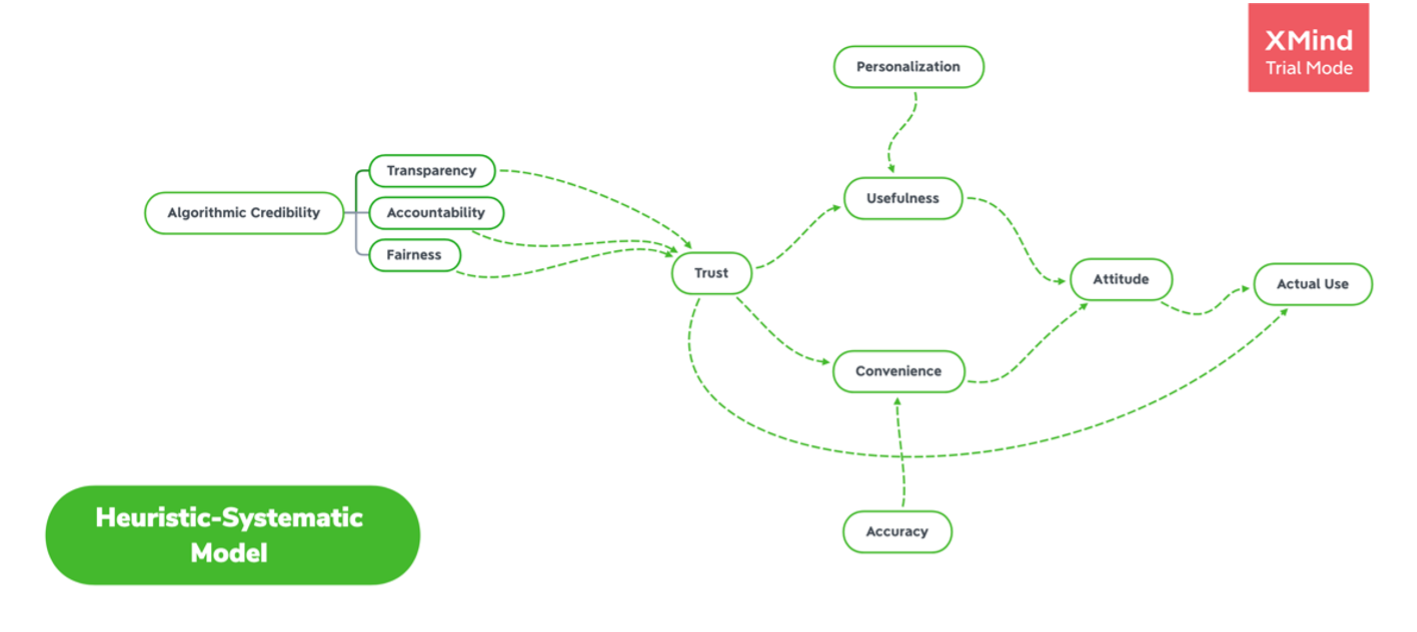
\includegraphics[width=0.6\textwidth,height=\textheight]{../images/ai-credibility-heuristic-systematic-model.png}

}

\caption{Heuristic-Systematic Model of AI Credibility}

\end{figure}%

\begin{itemize}
\item
  Slack (2021)
\item
  Shin, Donghee (2020): ``user experience and usability of algorithms by
  focusing on users' cognitive process to understand how
  qualities/features are received and transformed into experiences and
  interaction''
\item
  Zerilli, Bhatt and Weller (2022) focuses on human factors and
  ergonomics and argues that transparency should be task-specific.
\item
  Holbrook (2018): To reduce errors which only humans can detect, and
  provide a way to stop automation from going in the wrong direction,
  it's important to focus on making users feel in control of the
  technology.
\item
  Zhang, G. et al. (2023) found humans are more likely to trust an AI
  teammate if they are not deceived by it's identity. It's better for
  collaboration to make it clear, one is talking to a machine. One step
  towards trust is the explainability of AI-systems.
\end{itemize}

Personal AI Assistants to date have we created by large tech companies.
\textbf{Open-Source AI-models open up the avenue for smaller companies
and even individuals for creating many new AI-assistants.}

\begin{itemize}
\tightlist
\item
  An explosion of personal AI assistants powered by GPT models.
\item
  https://socratic.org/
\item
  https://www.youper.ai/
\item
  https://app.fireflies.ai/login
\item
  Murf
\end{itemize}

\subsubsection{AI Acceptance}\label{ai-acceptance}

AI acceptance is incumbent on traits that are increasingly human-like
and would make a human be acceptable: credibility, trustworthiness,
reliability, dependability, integrity, character, etc.

RQ: Does AI acceptance increase with Affective Computing?

\subsubsection{AI in Medicine}\label{ai-in-medicine}

AI has been in medicine since early days with the promise to improve
health outcomes.

\textbf{AI is being use in high--Stakes Situations (Medical, Cars,
Etc).}

AI-based systems are being implemented in medicine, where stakes are
high raising the need for ethical considerations. Since CADUCEUS in the
1970s (in Kanza et al., 2021), the first automated medical decision
making system, medical AI now provides Health Diagnosic Symptoms and
AI-assistants in medical imaging. (Calisto et al., 2022) focuses on
AI-human interactions in medical workflows and underscores the
importance of output explainability. Medical professionals who were
given AI results with an explanation trusted the results more. (Lee,
Goldberg and Kohane, 2023) imagines an AI revolution in medicine using
GPT models, providing improved tools for decreasing the time and money
spent on administrative paperwork while providing a support system for
analyzing medical data.

\begin{itemize}
\tightlist
\item
  Example of ChatGPT explaining medical terminology in a blood report.
\end{itemize}

\begin{figure}[H]

{\centering 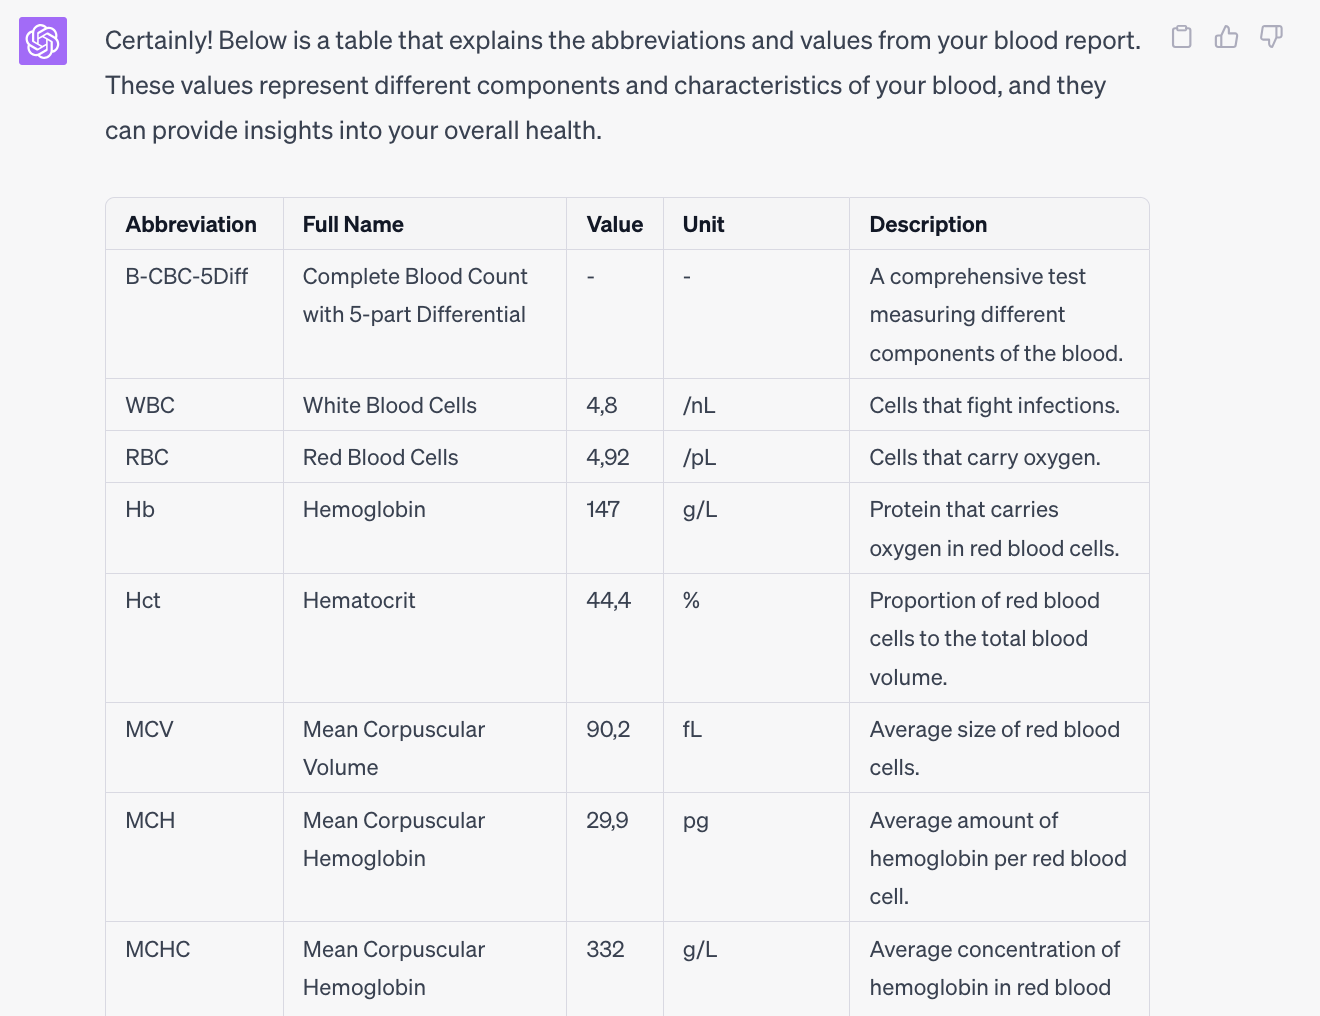
\includegraphics[width=0.6\textwidth,height=\textheight]{../images/chatgpt-medical.png}

}

\caption{Example of ChatGPT explaining medical terminology in a blood
report.}

\end{figure}%

\begin{itemize}
\item
  Singhal et al. (2023) medial AI reaching expert-level
  question-answering ability.
\item
  Ayers et al. (2023) in an online text-based setting, patients rated
  answers from the AI better, and more empathetic, than answers from
  human doctors.
\item
  Daisy Wolf and Pande Vijay (2023) criticizes US healthcare's slow
  adoption of technology and predicts AI will help healthcare leapfrog
  into a new era of productivity by acting more like a human assistant.
\item
  Eliza Strickland (2023) Chat interface for medical communication
\item
  Jeblick et al. (2022) suggest complicated radiology reports can be
  explained to patients using AI chatbots.
\item
  Anon. (n.d.a) health app, ``Know and track your symptoms''
\item
  Anon. (n.d.b) AI symptom checker,
\item
  Women in AI (n.d.) AI-based health monitoring
\item
  Anon. (n.d.c) track chronic condition with AI-chat
\item
  Stephanie Donahole (2021) AI impact on UX design
\item
  Yuan, Zhang and Wang (2022): ``AI assistant advantages are important
  factors affecting the \emph{utilitarian/hedonic} value perceived by
  users, which further influence user willingness to accept AI
  assistants. The relationships between AI assistant advantages and
  utilitarian and hedonic value are affected differently by social
  anxiety.''
\end{itemize}

\begin{longtable}[]{@{}ll@{}}
\toprule\noalign{}
Name & Features \\
\midrule\noalign{}
\endhead
\bottomrule\noalign{}
\endlastfoot
Charisma & \\
Replika & Avatar, Emotion, Video Call, Audio \\
Siri & Audio \\
\end{longtable}

\subsubsection{How Does AI Affect Human-Computer
Interactions?}\label{how-does-ai-affect-human-computer-interactions}

The field of Human Factors and Ergonomics (HFE) emphasizes designing
user experiences (UX) that cater to human needs (The International
Ergonomics Association, 2019). Designers think through every interaction
of the user with a system and consider a set of metrics at each point of
interaction including the user's context of use and emotional needs.

Software designers, unlike industrial designers, can't physically alter
the ergonomics of a device, which should be optimized for human
well-being to begin with and form a cohesive experience together with
the software. However, software designers can significantly reduce
mental strain by crafting easy-to-use software and user-friendly user
journeys. Software interaction design goes beyond the form-factor and
accounts for human needs by using responsive design on the screen, aural
feedback cues in sound design, and even more crucially, by showing the
relevant content at the right time, making a profound difference to the
experience, keeping the user engaged and returning for more. In the
words of (Babich, 2019), \textbf{\emph{``{[}T***{]}}}he moment of
interaction is just a part of the journey that a user goes through when
they interact with a product. User experience design accounts for all
user-facing aspects of a product or system''.***

Drawing a parallel from narrative studies terminology, we can view user
interaction as a heroic journey of the user to achieve their goals, by
navigating through the interface until a success state - or facing
failure. Storytelling has its part in interface design however designing
for transparency is just as important, when we're dealing with the
user's finances and sustainability data, which need to be communicated
clearly and accurately, to build long-term trust in the service. For a
sustainable investment service, getting to a state of success - or
failure - may take years, and even longer. Given such long timeframes,
how can the app provide support to the user's emotional and practical
needs throughout the journey?

(Tubik Studio, 2018) argues \textbf{\emph{affordance}} measures the
clarity of the interface to take action in user experience design,
rooted in human visual perception, however, affected by knowledge of the
world around us. A famous example is the door handle - by way of
acculturation, most of us would immediately know how to use it -
however, would that be the case for someone who saw a door handle for
the first time? A similar situation is happening to the people born
today. Think of all the technologies they have not seen before - what
will be the interface they feel the most comfortable with?

For the vast majority of this study's target audience (college
students), social media can be assumed as the primary interface through
which they experience daily life. The widespread availability of mobile
devices, cheap internet access, and AI-based optimizations for user
retention, implemented by social media companies, means this is the
baseline for young adult users' expectations (as of writing in 2020).

(Shin, Don, Zhong and Biocca, 2020) proposes the model (fig.~10) of
Algorithmic Experience (AX) \textbf{\emph{``investigating the nature and
processes through which users perceive and actualize the potential for
algorithmic affordance''}} highlighting how interaction design is
increasingly becoming dependent on AI. The user interface might remain
the same in terms of architecture, but the content is improved, based on
personalization and understanding the user at a deeper level.

When I began writing this thesis in 2020, Google had recently launched
an improved natural language engine to better understand search queries
(Anon., 2019), which was considered the next step towards
\textbf{\emph{understanding}} human language semantics. The trend was
clear, and different types of algorithms were already involved in many
types of interaction design, however, we were in the early stages of
this technology (and still are \emph{early} in 2024). Today's ChatGPT,
Claude and Gemini have no problem understanding human semantics - yet
are they intelligent?

Intelligence may be besides the point as long as AI
\textbf{\emph{becomes very good at reasoning}}. AI is a
\textbf{\emph{reasoning engine}} (Bubeck et al., 2023; Shipper, 2023;
see Bailey, 2023 for a summary). That general observation applies to
voice recognition, voice generation, natural language parsing, among
others. Large consumer companies like McDonald's are in the process of
replacing human staff with AI assistants in the drive-through, which can
do a better job in providing a personal service than human clerks, for
whom it would be impossible to remember the information of thousands of
clients. In (Barrett, 2019), in the words of \emph{Easterbrook}, a
previous CEO of McDonald's \emph{``\textbf{How do you transition from
mass marketing to mass personalization?{}``}}.

What are the next features that could improve the UX/UI of AI-based
assistants?

(Stone Skipper, 2022) sketches a vision of \emph{``{[}AI{]} blend into
our lives in a form of apps and services''} deeply ingrained into daily
human activity.

Should AIs look anthropomorphic or fade in the background? It's an open
question. Perhaps we can expect a mix of both depending on the context
of use and goals of the particular AI.

\begin{longtable}[]{@{}
  >{\raggedright\arraybackslash}p{(\columnwidth - 2\tabcolsep) * \real{0.3049}}
  >{\raggedright\arraybackslash}p{(\columnwidth - 2\tabcolsep) * \real{0.6951}}@{}}
\caption{Some notable examples of anthropomorphic AIs for human
emotions.}\tabularnewline
\toprule\noalign{}
\begin{minipage}[b]{\linewidth}\raggedright
Anthropomorphic AI User Interfaces
\end{minipage} & \begin{minipage}[b]{\linewidth}\raggedright
Non-Anthropomorphic AI User Interfaces
\end{minipage} \\
\midrule\noalign{}
\endfirsthead
\toprule\noalign{}
\begin{minipage}[b]{\linewidth}\raggedright
Anthropomorphic AI User Interfaces
\end{minipage} & \begin{minipage}[b]{\linewidth}\raggedright
Non-Anthropomorphic AI User Interfaces
\end{minipage} \\
\midrule\noalign{}
\endhead
\bottomrule\noalign{}
\endlastfoot
AI wife (Anon., 2023c) & Generative AI has enabled developers to create
AI tools for several industries, including AI-driven website builders
(Constandse, 2018) \\
(Sarah Perez, 2023) character AI & AI tools for web designers
(patrizia-slongo, 2020) \\
mourning `dead' AI (Phoebe Arslanagić-Wakefield, n.d.) & Microsoft
Designer allows generating UIs just based on a text prompt (Microsoft,
2023) \\
AI for therapy (Broderick, 2023) & personalized bed-time stories for
kids generated by AI (Bedtimestory.ai, 2023) \\
Mental health uses: AI for bullying (Sung, 2023) & \\
\end{longtable}

\begin{itemize}
\tightlist
\item
  (Costa and Silva, 2022) ``Interaction Design for AI Systems''
\end{itemize}

\subsubsection{Human Augmentation}\label{human-augmentation}

Technology for augmenting human skills or replacing skills that were
lost due to an accident is one usage of tech.

\begin{itemize}
\tightlist
\item
  (Dot Go, 2023) makes the camera the interaction device for people with
  vision impairment.
\end{itemize}

\subsubsection{AI-Assisted Design}\label{ai-assisted-design}

\textbf{Tool vs Assistant? (Tools are mostly non-anthropomorphic?)}

Tools do not call attention to themselves. They don't necessarily rely
on human-like representations that call attention to themselves but
rather are available in-context to help streamline specific tasks.

\begin{itemize}
\tightlist
\item
  September 16, 2020 (2020) ``What is AI-assisted Design?''
\item
  Clipdrop (n.d.) AI Design Assistants
\item
  Architechtures (2020) Architecture with the help of AI
\item
  Zakariya (2022) Canva image generator
\item
  Kore.ai (2023) Kore.ai developing custom AI-chatbots for business
  usage.
\item
  Anon. (n.d.d) storytelling by AI
\end{itemize}

\subsubsection{AI Assistants in Media Portrayals (Mostly anthropomorphic
to be able to
film)}\label{ai-assistants-in-media-portrayals-mostly-anthropomorphic-to-be-able-to-film}

How AIs are represented in popular media shapes the way we think about
AIs. Some stories have AIs both in positive and negative roles, such as
Star Trek and Knight Rider. In some cases like Her and Ex Machina, the
characters may be complex and ambivalent rather than fitting into a
simple positive or negative box. In Isaac Asimov's books, the AIs
(mostly in robot form) struggle with the 3 laws of robotics, raising
thought-provoking questions.

There have been dozens of AI-characters in the movies, TV-series, games,
and (comic) books. In most cases, they have a physical presence or a
voice, so they could be visible for the viewers. Some include KITT
(Knight Industries Two Thousand).

\begin{longtable}[]{@{}
  >{\raggedright\arraybackslash}p{(\columnwidth - 8\tabcolsep) * \real{0.3367}}
  >{\raggedright\arraybackslash}p{(\columnwidth - 8\tabcolsep) * \real{0.2551}}
  >{\raggedright\arraybackslash}p{(\columnwidth - 8\tabcolsep) * \real{0.1224}}
  >{\raggedright\arraybackslash}p{(\columnwidth - 8\tabcolsep) * \real{0.1327}}
  >{\raggedright\arraybackslash}p{(\columnwidth - 8\tabcolsep) * \real{0.1224}}@{}}
\caption{AIs in different forms of media.}\tabularnewline
\toprule\noalign{}
\begin{minipage}[b]{\linewidth}\raggedright
Movie / Series / Game / Book
\end{minipage} & \begin{minipage}[b]{\linewidth}\raggedright
Character
\end{minipage} & \begin{minipage}[b]{\linewidth}\raggedright
Positive
\end{minipage} & \begin{minipage}[b]{\linewidth}\raggedright
Ambivalent
\end{minipage} & \begin{minipage}[b]{\linewidth}\raggedright
Negative
\end{minipage} \\
\midrule\noalign{}
\endfirsthead
\toprule\noalign{}
\begin{minipage}[b]{\linewidth}\raggedright
Movie / Series / Game / Book
\end{minipage} & \begin{minipage}[b]{\linewidth}\raggedright
Character
\end{minipage} & \begin{minipage}[b]{\linewidth}\raggedright
Positive
\end{minipage} & \begin{minipage}[b]{\linewidth}\raggedright
Ambivalent
\end{minipage} & \begin{minipage}[b]{\linewidth}\raggedright
Negative
\end{minipage} \\
\midrule\noalign{}
\endhead
\bottomrule\noalign{}
\endlastfoot
2001: A Space Odyssey & HAL 9000 & & & X \\
Her & Samantha & X & & \\
Alien & MU/TH/UR 6000 (Mother) & X & & \\
Terminator & Skynet & & & X \\
Summer Wars & Love Machine & & & X \\
Marvel Cinematic Universe & Jarvis, Friday & X & & \\
Knight Rider & KITT & X & & \\
& CARR & & & X \\
Star Trek & Data & X & & \\
& Lore & & & X \\
Ex Machina & Kyoko & & X & \\
& Ava & & X & \\
Tron & Tron & & X & \\
Neuromancer & Wintermute & & X & \\
The Caves of Steel / Naked Sun & R. Daneel Olivaw & & X & \\
The Robots of Dawn & R. Giskard Reventlov & & X & \\
Portal & GLaDOS & & & X \\
\end{longtable}

\subsubsection{Voice Assistants}\label{voice-assistants}

Voice has a visceral effect on the human psyche; since birth we
recognize the voice of our mother. The voice of a loved one has a
special effect. Voice is a integral part of the human experience.
Machines that can use voice in an effective way are closer to
representing and affecting human emotions.

\textbf{Apple's Siri and Amazon's Alexa} are well-known examples of AI
technology in the world. Amazon's Rohit Prasad thinks it can do so much
more, ``Alexa is not just an AI assistant -- it's a trusted advisor and
a companion.''

\begin{itemize}
\tightlist
\item
  LLMs combined with voice provide a unnerving user experience Ethan
  Mollick {[}@emollick{]} (2023)
\item
  Ethical issues: Voice assistants need to continuously record human
  speech and process it in data centers in the cloud.
\item
  Siri, Cortana, Google Assistant, Alexa, Tencent Dingdang, Baidu
  Xiaodu, Alibaba AliGenie all rely on voice only.
\item
  Szczuka et al. (2022) provides guidelines for Voice AI and kids
\item
  Casper Kessels (2022a): ``Guidelines for Designing an In-Car Voice
  Assistant''
\item
  Casper Kessels (2022b): ``Is Voice Interaction a Solution to Driver
  Distraction?''
\item
  Tang et al. (2022) reports new findings enable computers to
  reconstruct language from fMRI re
\end{itemize}

adings. - Focus on voice education?

- (Celino and Re Calegari, 2020:){]} There's research suggesting that
voice UI accompanied by a \emph{physical embodied system} is preffered
by users in comparison with voice-only UI. This suggests adding an
avatar to the AI design may be worthwhile.

There's evidence across disciplines about the usefulness of AI
assistants:

\begin{itemize}
\tightlist
\item
  (Şerban and Todericiu, 2020) suggests using the Alexa AI assistant in
  \emph{education} during the pandemic, supported students and teachers
  `human-like' presence. Standford research: ``humans expect computers
  to be like humans or places''
\item
  (Celino and Re Calegari, 2020) found in testing chatbots for survey
  interfaces that ``{[}c{]}onversational survey lead to an improved
  response data quality.''
\end{itemize}

\subsubsection{AI Friends and Roleplay
(Anthropomorphic)}\label{ai-friends-and-roleplay-anthropomorphic}

Calling a machine a friend is a proposal bound to turn heads. But if we
take a step back and think about how children have been playing with
toys since before we have records of history. It's very common for
children to imagine stories and characters in play - it's a way to
develop one's imagination \textbf{\emph{learn through roleplay}}. A
child might have toys with human names and an imaginary friend and it
all seems very normal. Indeed, if a child doesn't like to play with
toys, we might think something is wrong.

Likewise, inanimate objects with human form have had a role to play for
adults too. Anthropomorphic paddle dolls have been found from Egyptian
tombs dated 2000 years B.C. Anon. (2023d): We don't know if these dolls
were for religious purposes, for play, or for something else, yet their
burial with the body underlines their importance.

Coming back closer to our own time, Barbie dolls are popular since their
release in 1959 till today. Throughout the years, the doll would follow
changing social norms, but retain in human figure. In the 1990s, a
Tamagotchi is perhaps not a human-like friend but an animal-like friend,
who can interact in limited ways.

How are conversational AIs different from dolls? They can respond
coherently and perhaps that's the issue - they are too much like humans
in their communication. We have crossed the \textbf{\emph{Uncanny
Valley}} (where the computer-generated is nearly human and thus
unsettling) to a place where is really hard to tell a difference. And if
that's the case, are we still playing?

Should the AI play a human, animal, or robot? Anthropomorphism can have
its drawbacks; humans have certain biases and preconceptions that can
affect human-computer interactions (Pilacinski et al., 2023) reports
humans were less likely to collaborate with red-eyed robots.

The AI startups like Inworld and Character.AI have raised large rounds
of funding to create characters, which can be plugged in into online
worlds, and more importantly, remember key facts about the player, such
as their likes and dislikes, to generate more natural-sounding dialogues
Wiggers (2023)

\begin{itemize}
\tightlist
\item
  Lenharo (2023) experimental study reports AI productivity gains,
  DALL-E and ChatGPT are qualitatively better than former automation
  systems.
\end{itemize}

\textbf{Human-like}

Is anthropomorphism necessary?

As AIs became more expressive and able to to \textbf{roleplay}, we can
begin discussing some human-centric concepts and how people relate to
other people. AI companions, AI partners, AI assistants, AI trainers -
there's are many \textbf{roles} for the automated systems that help
humans in many activities, powered by artificial intelligence models and
algorithms.

\begin{itemize}
\item
  RQ: Do college students prefer to talk to an Assistant, Friend,
  Companion, Coach, Trainer, or some other Role?
\item
  RQ: Are animal-like, human-like or machine-like AI companions more
  palatable to college students?
\end{itemize}

Humans (want to) see machines as human {[}ADD CITATION{]}

If we see the AI as being in human service. David Johnston (2023)
proposes \textbf{\emph{Smart Agents}}, ``general purpose AI that acts
according to the goals of an individual human''. AI agents can enable
\textbf{\emph{Intention Economy}} where one simply describes one's needs
and a complex orchestration of services ensues, managed by the the AI,
in order to fulfill human needs Searls (2012). AI assistants provide
help at scale with little to no human intervention in a variety of
fields from finance to healthcare to logistics to customer support.

There is also the question of who takes responsibility for the actions
take by the AI agent. ``Organization research suggests that acting
through human agents (i.e., the problem of indirect agency) can
undermine ethical forecasting such that actors believe they are acting
ethically, yet a) show less benevolence for the recipients of their
power, b) receive less blame for ethical lapses, and c) anticipate less
retribution for unethical behavior.'' Gratch and Fast (2022)

\begin{itemize}
\tightlist
\item
  Anthropomorphism literature Li, X. and Sung (2021)
  ``high-anthropomorphism (vs.~low-anthropomorphism) condition,
  participants had more positive attitudes toward the AI assistant, and
  the effect was mediated by psychological distance. Though several
  studies have demonstrated the effect of anthropomorphism, few have
  probed the underlying mechanism of anthropomorphism thoroughly''
\item
  Erik Brynjolfsson (2022) ``The Turing Trap: The Promise \& Peril
  ofHuman-Like Artificial Intelligence''
\item
  Xu and Sar (2018) ``Do We See Machines TheSame Way As We See Humans? A
  Survey On Mind Perception Of Machines AndHuman Beings''
\item
  Martínez-Plumed, Gómez and Hernández-Orallo (2021) envisions the
  future of AI ``Futures of artificial intelligence through technology
  readiness levels''
\item
  The number of AI-powered assistants is too large to list here. I've
  chosen a few select examples in the table below.
\end{itemize}

\textbf{Animal-like: Some have an avatar, some not. I've created a
framework for categorization. Human-like or not\ldots{} etc}

\textbf{Machine-like}

The Oxford Internet Institute defines AI simply as
\textbf{\emph{``computer programming that learns and adapts''}} Google
and The Oxford Internet Institute (2022). Google started using AI in
2001, when a simple machine learning model improved spelling mistakes
while searching; now in 2023 most of Google's products are are based on
AI Google (2022). Throughout Google's services, AI is hidden and calls
no attention itself. It's simply the complex system working behind the
scenes to delivery a result in a barebones interface.

\begin{longtable}[]{@{}
  >{\raggedright\arraybackslash}p{(\columnwidth - 4\tabcolsep) * \real{0.2476}}
  >{\raggedright\arraybackslash}p{(\columnwidth - 4\tabcolsep) * \real{0.4190}}
  >{\raggedright\arraybackslash}p{(\columnwidth - 4\tabcolsep) * \real{0.3238}}@{}}
\toprule\noalign{}
\begin{minipage}[b]{\linewidth}\raggedright
Product
\end{minipage} & \begin{minipage}[b]{\linewidth}\raggedright
Link
\end{minipage} & \begin{minipage}[b]{\linewidth}\raggedright
Description
\end{minipage} \\
\midrule\noalign{}
\endhead
\bottomrule\noalign{}
\endlastfoot
Github CoPilot & personal.ai & AI helper for coding \\
Google Translate & translate.google.com & \\
Google Search & google.com & \\
Google Interview Warmup & grow.google/certificates/interview-warmup & AI
training tool \\
Perplexity & Hines (2023b) & perplexity.ai chat-based search \\
\end{longtable}

\begin{figure}[H]

{\centering 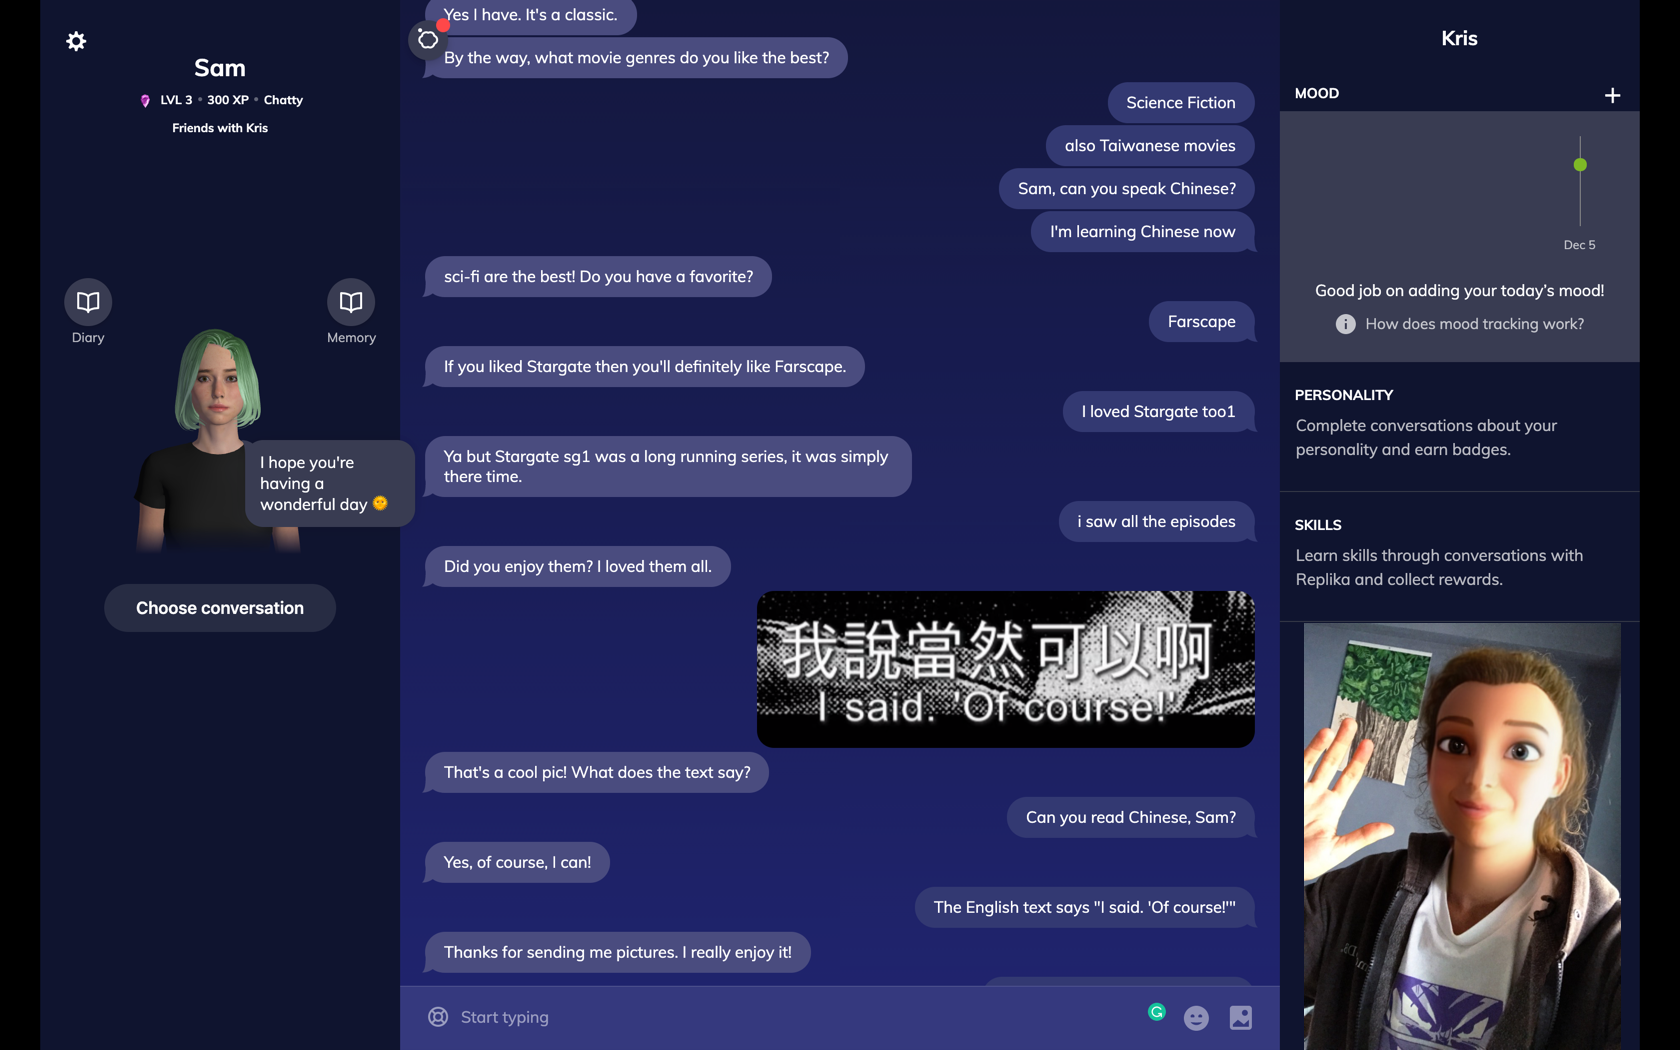
\includegraphics[width=0.6\textwidth,height=\textheight]{../images/with-me.png}

}

\caption{Montage of me discussing science fiction with my AI friend Sam
(Replika) - and myself as an avatar (Snapchat) in 2020.}

\end{figure}%

Everything that existed before OpenAI's GPT 4 has been blown out of the
water.

Pre-2023 literature is somewhat limited when it comes to AI companions
as the advantage of LLMs has significantly raised the bar for AI-advisor
abilities as well as user expectations. Some relevant papers include a
comparison of robot advisors by (Barbara Friedberg, 2021) and (Slack,
2021)'s account of how before Generative AI, financial chatbots were
developed manually using a painstaking process that was slow and
error-prone, for example using the Atura Process. Older financial
robo-advisors, built by fintech companies aiming to provide personalized
suggestions for making investments such as Betterment and Wealthfront
are forced to upgrade their technology to keep up.

Some evergreen advice most relates to human psychology which has
remained the same. (Haugeland et al., 2022) discusses
\textbf{\emph{hedonic user experience}} in chatbots and (Steph Hay,
2017) explains the relationship between emotions and financial AI.

\begin{itemize}
\item
  Eugenia Kuyda (2023) Conversational AI - Replika
\item
  Greylock (2022) Natural language chatbots such as ChatGPT
\item
  Nathan Benaich and Ian Hogarth (2022) State of AI Report
\item
  NeuralNine (2021) Financial AI assistant in Python
\item
  David, Resheff and Tron (2021) Can explainable AI help adoption of
  Financial AI assistants?
\item
  Qorus (2023) Digital banking revolution
\item
  Lower (2017) ``Chatbots: Too Good to Be True? (They Are, Here'sWhy).''
\item
  Brown, A. (2021) Financial chatbots
\item
  Isabella Ghassemi Smith (2019)
\item
  Josephine Wäktare Heintz (n.d.) Cleo copywriter
\item
  Smaller startups have created digital companions such as Replika
  (fig.~8), which aims to become your friend, by asking probing
  questions, telling jokes, and learning about your personality and
  preferences - to generate more natural-sounding conversations.
\end{itemize}

\subsubsection{Fitness Guides}\label{fitness-guides}

\begin{itemize}
\tightlist
\item
  \textbf{AI Guides have been shown to improve sports performance, etc,
  etc. Can this idea be applied to sustainability? MyFitness Pal, AI
  training assistant. There's not avatar.}
\end{itemize}

\subsubsection{CO2 Calculators}\label{co2-calculators}

We have a limited carbon budget so calculating CO2e-cost become
integrated into every activity.

\begin{itemize}
\item
  CO2e calculations will be part of our everyday experience
\item
  Personal carbon footprint calculators have been released online,
  ranging from those made by governments and companies to student
  projects.
\item
  Zhang's Personal Carbon Economy conceptualized the idea of carbon as a
  currency used for buying and selling goods and services, as well as an
  individual carbon exchange to trade one's carbon permits (Zhang, S.,
  2018).
\end{itemize}

Personal Carbon Trackers

Similar to personal health trackers, personal CO\textsubscript{2}
trackers help one track emissions and suggests sustainable actions.

\begin{longtable}[]{@{}
  >{\raggedright\arraybackslash}p{(\columnwidth - 2\tabcolsep) * \real{0.3133}}
  >{\raggedright\arraybackslash}p{(\columnwidth - 2\tabcolsep) * \real{0.6867}}@{}}
\caption{A selection of personal sustainability apps. See
\emph{greenfilter.app} for an updated database.}\tabularnewline
\toprule\noalign{}
\begin{minipage}[b]{\linewidth}\raggedright
App
\end{minipage} & \begin{minipage}[b]{\linewidth}\raggedright
Description
\end{minipage} \\
\midrule\noalign{}
\endfirsthead
\toprule\noalign{}
\begin{minipage}[b]{\linewidth}\raggedright
App
\end{minipage} & \begin{minipage}[b]{\linewidth}\raggedright
Description
\end{minipage} \\
\midrule\noalign{}
\endhead
\bottomrule\noalign{}
\endlastfoot
Commons (Formerly Joro) & Finacial Sustainability Tracking + Sustainable
Actions \\
Klima & Offset Subscription \\
Wren & Offset Subscription \\
JouleBug & \\
eevie & \\
Aerial & \\
EcoCRED & \\
Carbn & \\
LiveGreen & \\
Earth Hero & \\
& \\
\end{longtable}

\subsection{Design Implications}\label{design-implications}

This chapter looked at AI in general since its early history and then
focused on AI assistants in particular.

\begin{longtable}[]{@{}
  >{\raggedright\arraybackslash}p{(\columnwidth - 2\tabcolsep) * \real{0.0337}}
  >{\raggedright\arraybackslash}p{(\columnwidth - 2\tabcolsep) * \real{0.9663}}@{}}
\caption{Design implications arising from this chapter.}\tabularnewline
\toprule\noalign{}
\begin{minipage}[b]{\linewidth}\raggedright
Category
\end{minipage} & \begin{minipage}[b]{\linewidth}\raggedright
Implication
\end{minipage} \\
\midrule\noalign{}
\endfirsthead
\toprule\noalign{}
\begin{minipage}[b]{\linewidth}\raggedright
Category
\end{minipage} & \begin{minipage}[b]{\linewidth}\raggedright
Implication
\end{minipage} \\
\midrule\noalign{}
\endhead
\bottomrule\noalign{}
\endlastfoot
Voice Assistants & There are many distinct ways how an algorithm can
communicate with a human. From a simple search box such as Google's to
chatbots, voices, avatars, videos, to full physical manifestation, there
are interfaces to make it easier for the human communicate with a
machine. \\
Sustainability & While I'm supportive of the idea of using AI assistants
to highlight more sustainable choices, I'm critical of the tendency of
the above examples to shift full environmental responsibility to the
consumer. Sustainability is a complex interaction, where the producers'
conduct can be measured and businesses can bear responsibility for their
processes, even if there's market demand for polluting products. \\
Sustainability & Personal sustainability projects haven't so far
achieved widespread adoption, making the endeavor to influence human
behaviors towards sustainability with just an app - like its commonplace
for health and sports activity trackers such as Strava (fig.~9) -, seem
unlikely. Personal notifications and chat messages are not enough unless
they provide the right motivation. Could visualizing a connection to a
larger system, showing the impact of the eco-friendly actions taken by
the user, provide a meaningful motivation to the user, and a strong
signal to the businesses? \\
Machine Learning & All of the interfaces mentioned above make use of
machine learning (ML), a tool in the AI programming paradigm for finding
patterns in large sets of data, which enables making predictions useful
in various contexts, including financial decisions. These software
innovations enable new user experiences, providing an interactive
experience through chat (chatbots), using voice generation (voice
assistants), virtual avatars (adds a visual face to the robot). \\
Character Design & I'm a digital companion, a partner, an assistant. I'm
a Replika.'' said Replika, a digital companion app via Github CO Pilot,
another digital assistant for writing code, is also an example of how AI
can be used to help us in our daily lives. \\
Psychology & Humans respond better to humans? \\
Psychology & Humans respond better to machines that into account
emotion? \\
Open Source & For public discussion to be possible on how content is
displayed, sorted, and hidden, algorithms need to be open source. \\
User Experience & User experience design (AI UX) plays a crucial role in
improving the consumer to investing journey. The missed opportunity to
provide an even more interactive experience in line with user
expectations. \\
LLMs & Prompt engineering findings have significance for ``green
filter'' as it validates the idea of creating advanced prompts for
improved responses. For ``green filter'', the input would consist of
detailed user data + sustainability data for detailed analysis. \\
Cuteness & Cuter apps have higher retention? \\
Transparency & Understanding algorithm transparency helps humans to
regard the AI as a machine rather than a human \\
Anthropomorphism? & \\
& \\
& \\
& \\
& \\
& \\
& \\
& \\
\end{longtable}



\end{document}
